\makeatletter
% Legendas de longtable no mesmo estilo do modelo SBC (Helvetica 10 pt, negrito)
\def\LT@makecaption#1#2#3{%
  \LT@mcol\LT@cols c{\hbox to\z@{\hss\parbox[t]\LTcapwidth{%
    \centering\sffamily\captionsize\textbf{#2. #3}\par\vskip\belowcaptionskip}\hss}}}
\makeatother
\setlength{\LTcapwidth}{\textwidth}
\setlength{\LTpre}{6pt}
\setlength{\LTpost}{6pt}

\newcommand{\pendente}[1]{\textcolor{red}{\textbf{[PENDENTE: #1]}}}
\newcommand{\repo}{\url{https://github.com/lipe0312/eventos-mata60}}
\DeclareUrlCommand\cod{\urlstyle{tt}}
\makeatletter
\g@addto@macro\UrlBreaks{\do\_\do\(\do\)\do\,}
\Urlmuskip=0mu plus 2mu
\makeatother
\newcolumntype{L}[1]{>{\raggedright\arraybackslash}p{#1}}
\newcolumntype{Y}{>{\raggedright\arraybackslash}X}

\lstdefinestyle{sql}{
  language=SQL,
  basicstyle=\ttfamily\footnotesize,
  keywordstyle=\bfseries,
  columns=fullflexible,
  keepspaces=true,
  frame=tb,
  framerule=0.4pt,
  aboveskip=6pt,
  belowskip=6pt,
  showstringspaces=false,
  breaklines=true,
  morekeywords={GENERATED,ALWAYS,IDENTITY,DEFERRABLE,INITIALLY,DEFERRED,TRIGGER,EXECUTE,FUNCTION,RECURSIVE,ATOMIC,PROCEDURE,ROLE,GRANT,USAGE,SCHEMA}
}
\lstset{style=sql}

\renewcommand{\arraystretch}{1.15}

% Figuras do MER, já recortadas em PDF vetorial e nomeadas pelo número no relatório.
% Foram geradas a partir das exportações do brModelo (mer-final.pdf, VF2, e mer-v1.pdf),
% com trim = esquerda inferior direita superior, em pontos:
%   figura-1-2-mer-v1        28 30 28 30            (mer-v1)
%   figura-1-3-mer-geral     35 36 83 36            (mer-final)
%   figura-1-4-mer-parte-a   26.2 37.3 547.4 281.5  (mer-final)
%   figura-1-5-mer-parte-b   278.2 68.1 220.1 278.2 (mer-final)
%   figura-1-6-mer-parte-c   49.1 303.7 357.6 68.7  (mer-final)
%   figura-1-7-mer-parte-d   428.7 192.4 114.1 94.9 (mer-final)
%   figura-1-8-mer-parte-e   526.9 225.1 76.1 32.7  (mer-final)
%   figura-1-9-mer-parte-f   418.9 37.3 76.1 402.5  (mer-final)
\newcommand{\mervum}{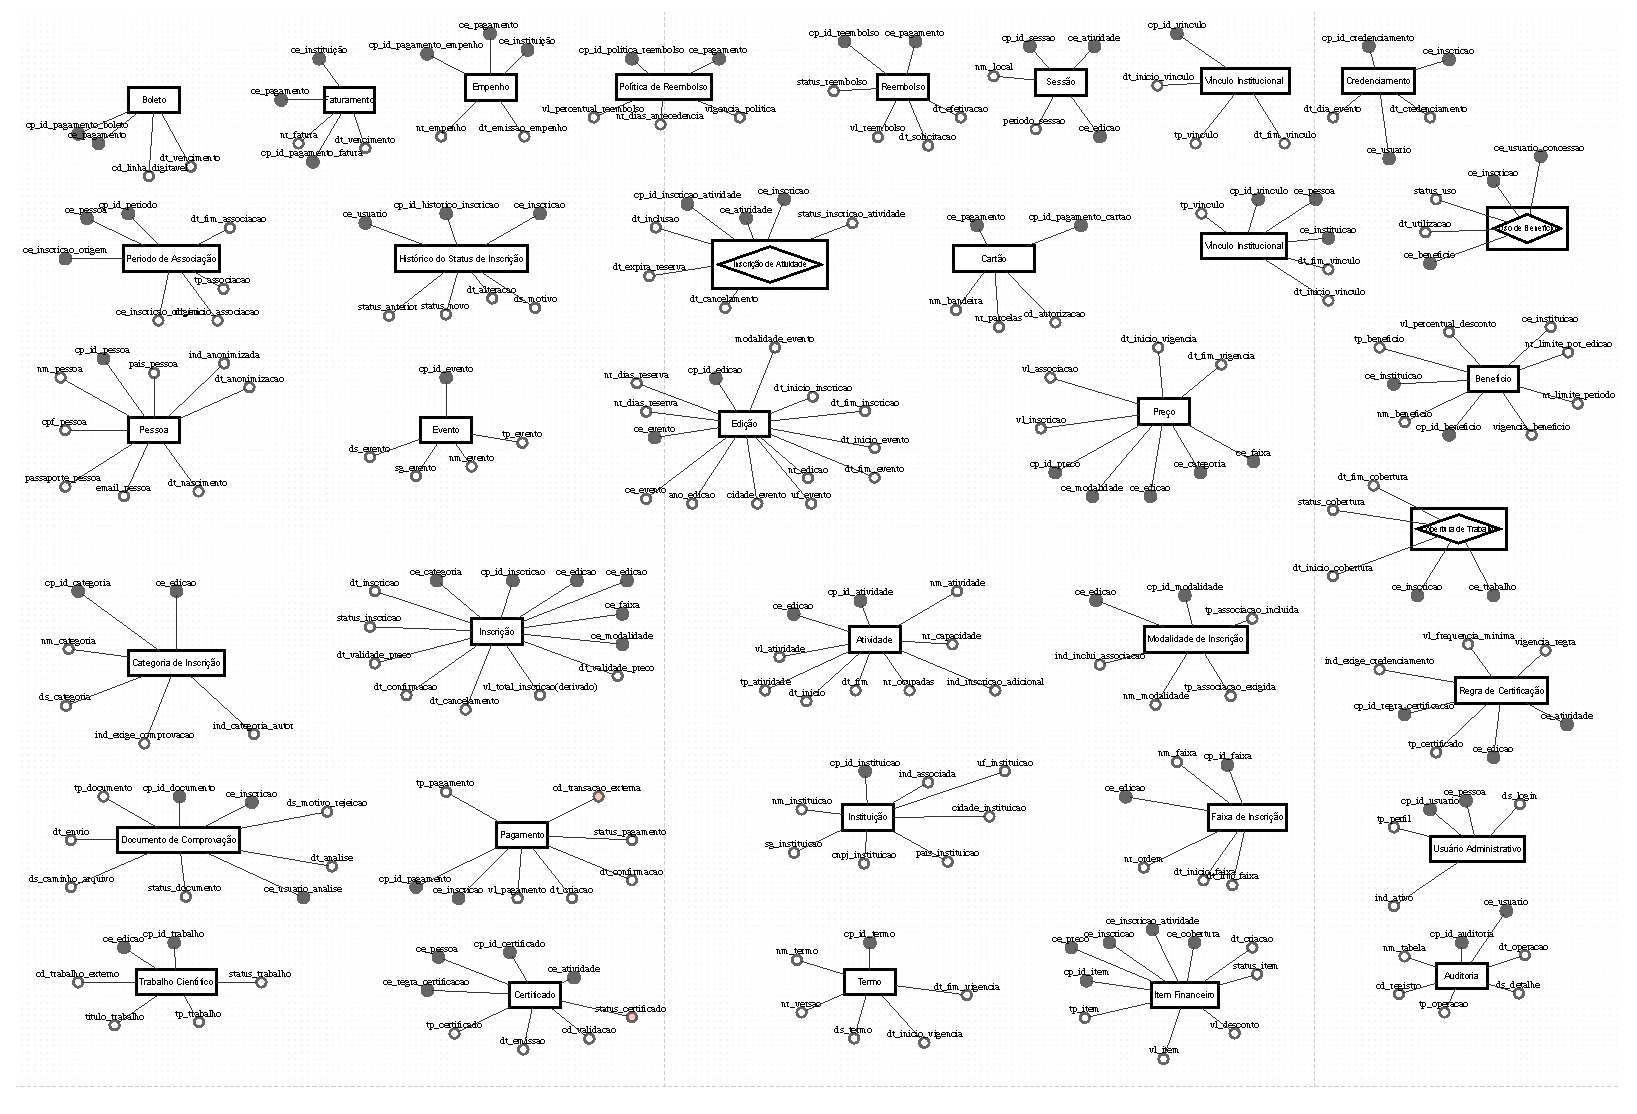
\includegraphics[width=\linewidth]{figura-1-2-mer-v1}}
\newcommand{\mergeral}{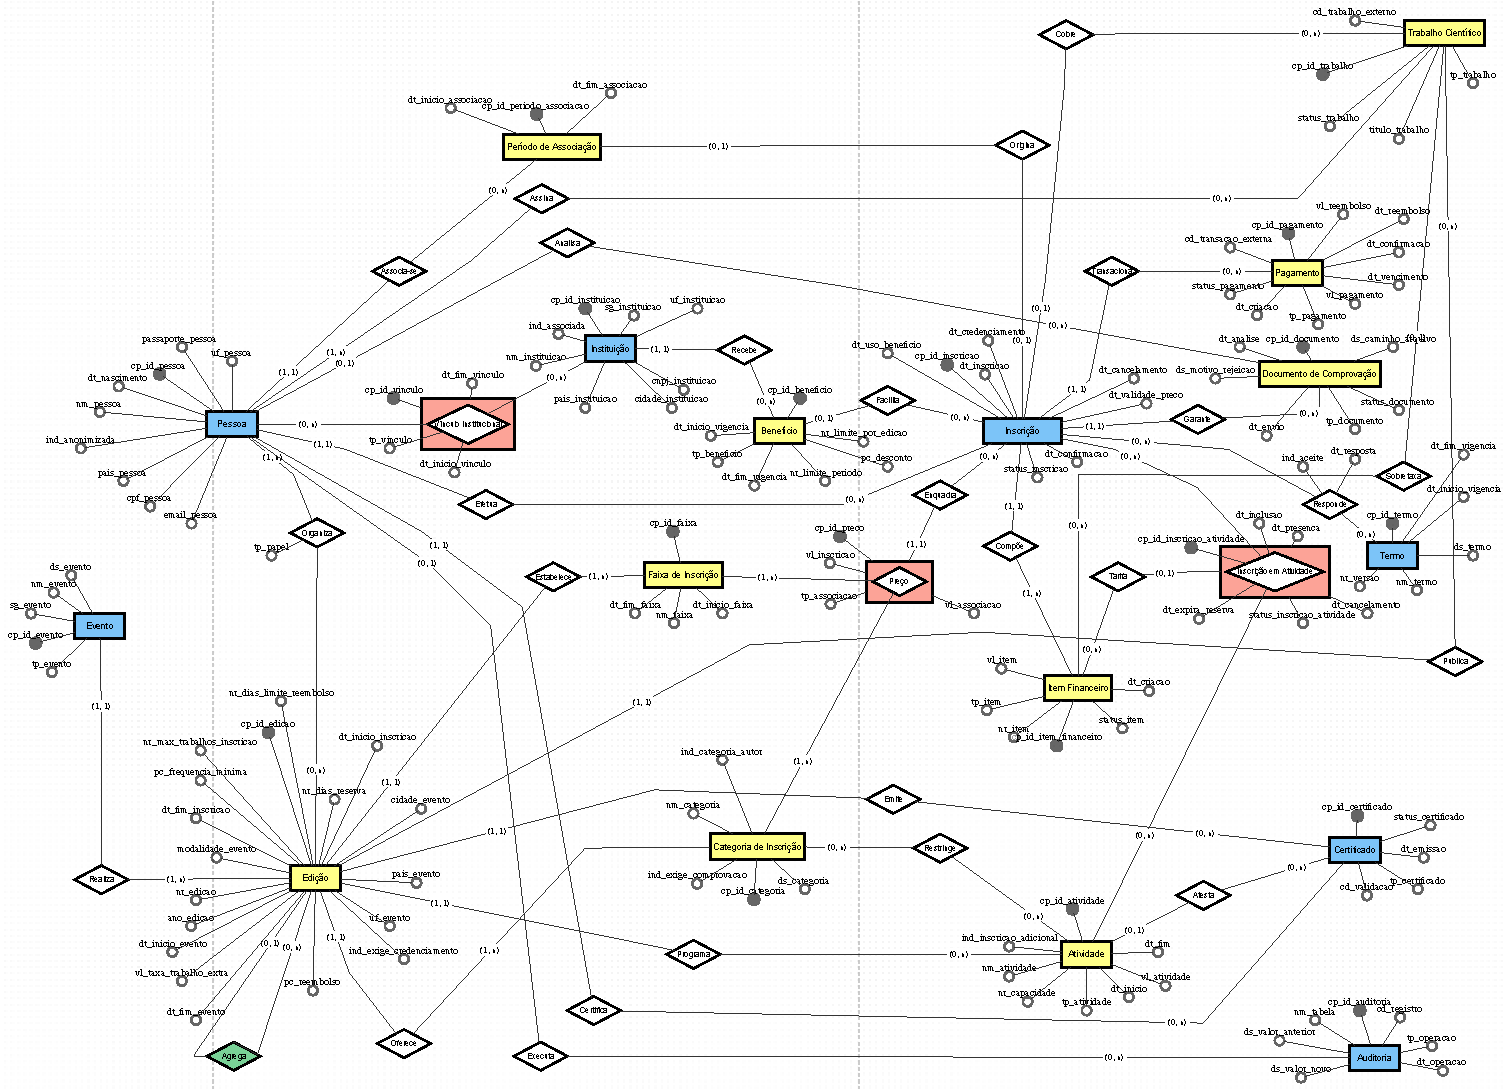
\includegraphics[width=\linewidth,height=0.97\textheight,keepaspectratio]{figura-1-3-mer-geral}}
\newcommand{\merA}{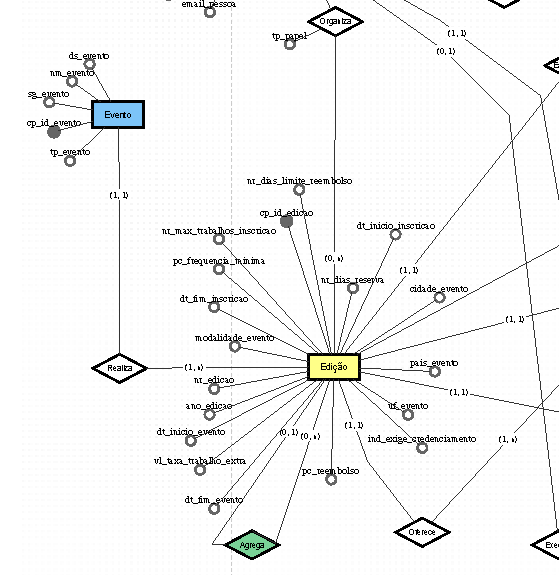
\includegraphics[width=0.78\linewidth]{figura-1-4-mer-parte-a}}
\newcommand{\merB}{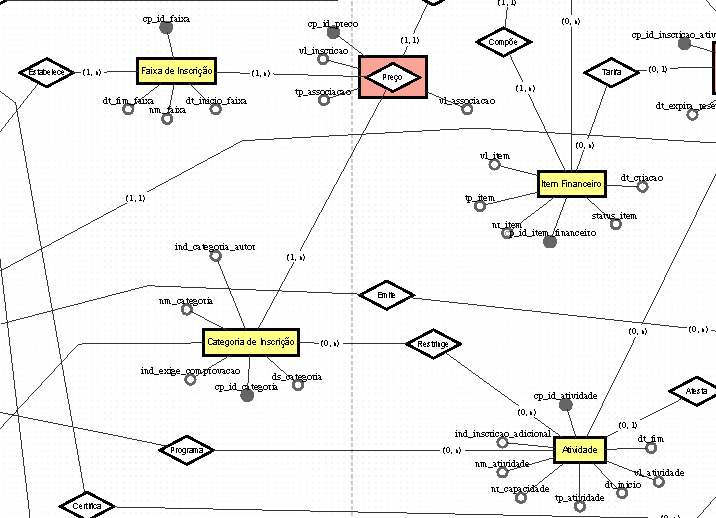
\includegraphics[width=\linewidth]{figura-1-5-mer-parte-b}}
\newcommand{\merC}{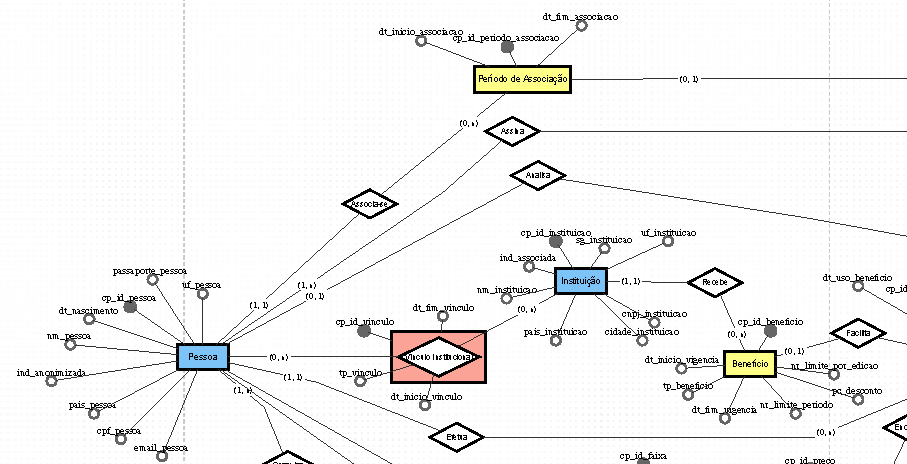
\includegraphics[width=\linewidth]{figura-1-6-mer-parte-c}}
\newcommand{\merD}{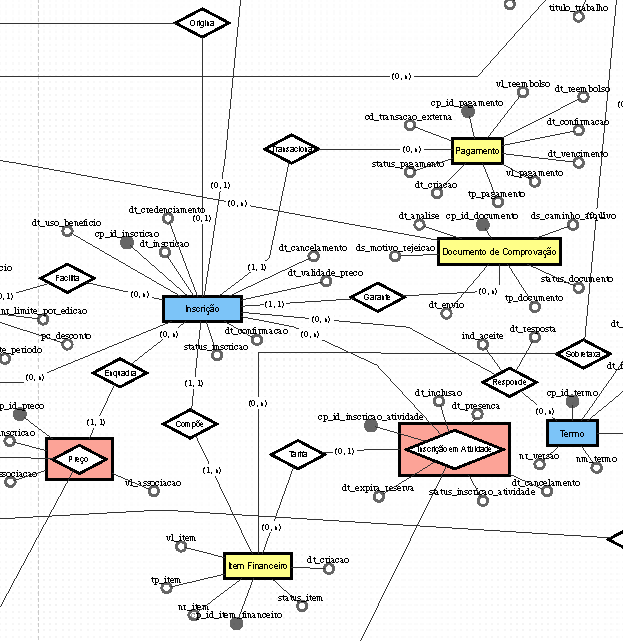
\includegraphics[width=0.9\linewidth]{figura-1-7-mer-parte-d}}
\newcommand{\merE}{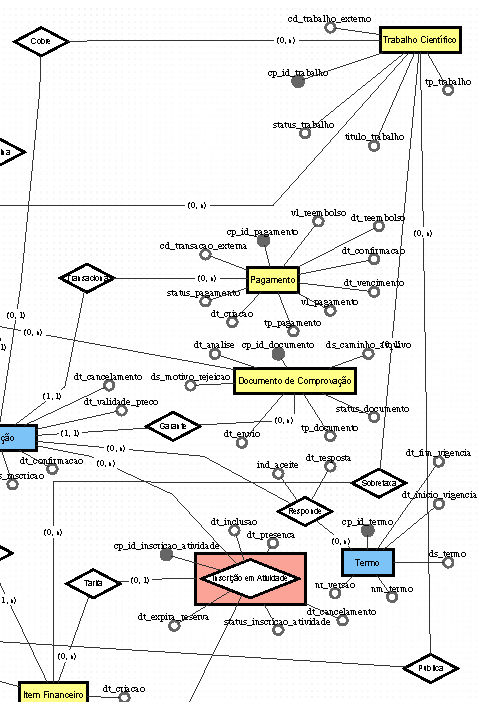
\includegraphics[width=0.7\linewidth]{figura-1-8-mer-parte-e}}
\newcommand{\merF}{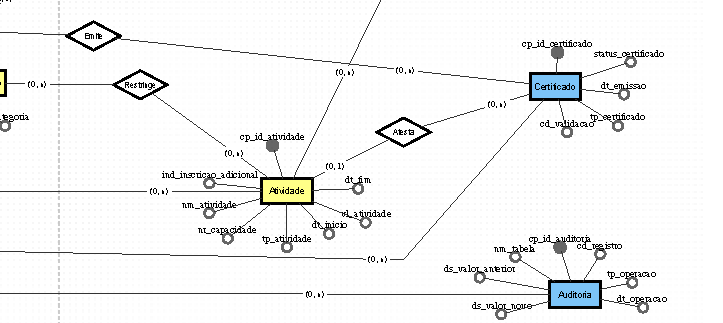
\includegraphics[width=\linewidth]{figura-1-9-mer-parte-f}}

% Figuras do modelo lógico, recortadas de logico-final.pdf (exportação VF do brModelo), trim em pontos:
%   figura-1-10-logico-geral    34 36 187 35
%   figura-1-11-logico-parte-a  32.7 297.1 573.6 49.1
%   figura-1-12-logico-parte-b  219.3 346.2 380.5 68.7
%   figura-1-13-logico-parte-c  45.8 85.7 645.6 297.8
%   figura-1-14-logico-parte-d  265.1 143.3 370.6 288.0
%   figura-1-15-logico-parte-e  209.5 32.1 344.5 441.8
%   figura-1-16-logico-parte-f  448.4 280.8 190.6 32.7
%   figura-1-17-logico-parte-g  490.9 149.9 187.4 343.6
\newcommand{\loggeral}{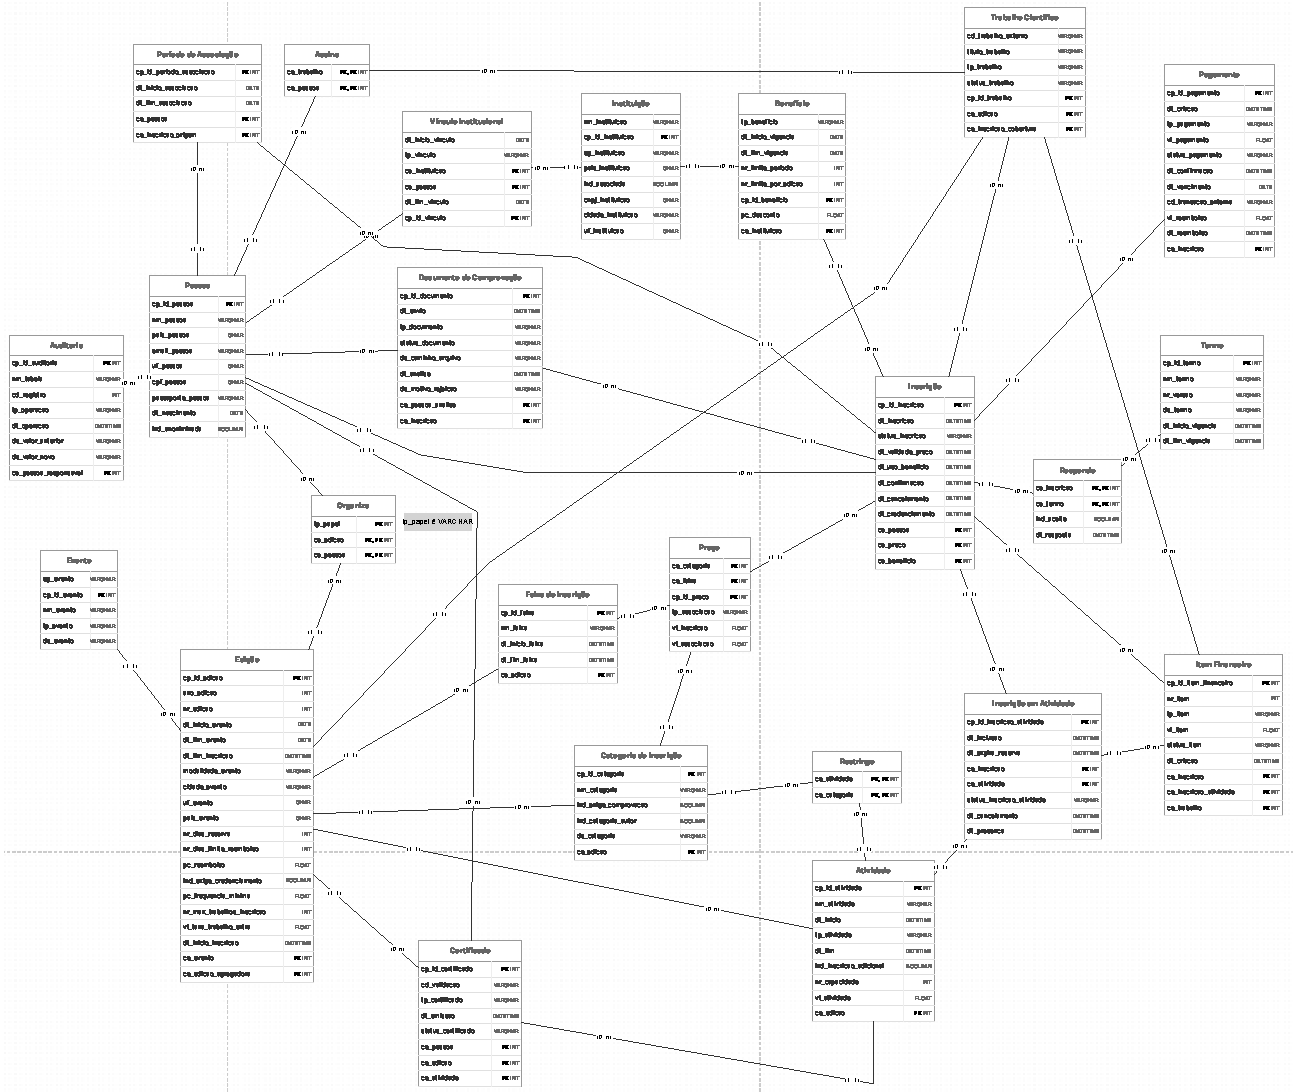
\includegraphics[width=\linewidth,height=0.97\textheight,keepaspectratio]{figura-1-10-logico-geral}}
\newcommand{\logA}{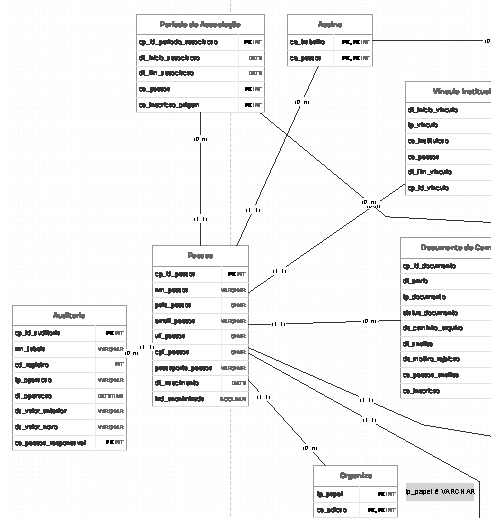
\includegraphics[width=0.95\linewidth]{figura-1-11-logico-parte-a}}
\newcommand{\logB}{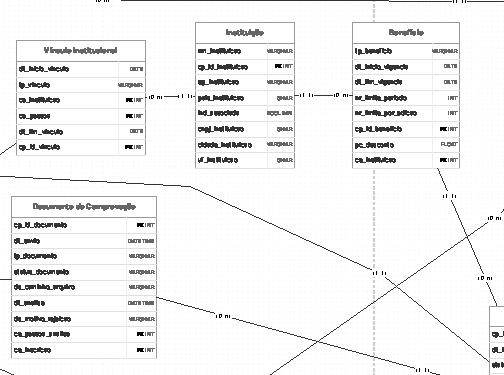
\includegraphics[width=\linewidth]{figura-1-12-logico-parte-b}}
\newcommand{\logC}{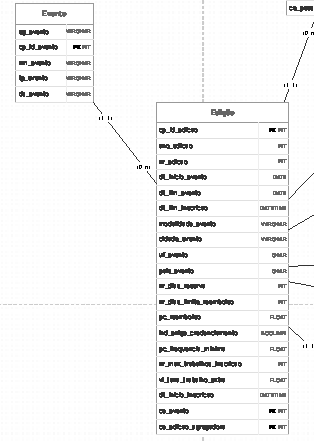
\includegraphics[width=0.6\linewidth]{figura-1-13-logico-parte-c}}
\newcommand{\logD}{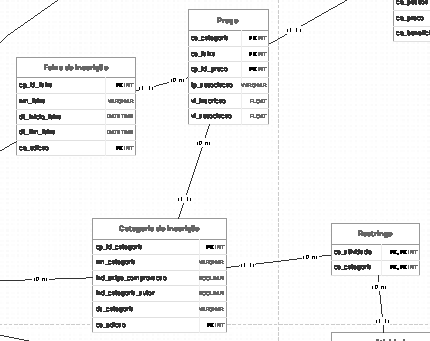
\includegraphics[width=0.82\linewidth]{figura-1-14-logico-parte-d}}
\newcommand{\logE}{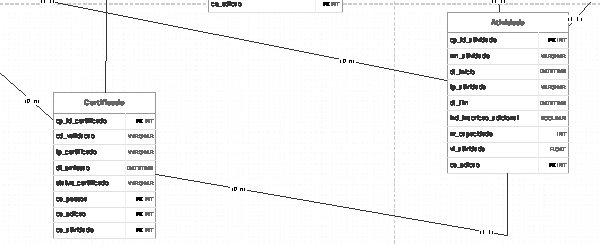
\includegraphics[width=\linewidth]{figura-1-15-logico-parte-e}}
\newcommand{\logF}{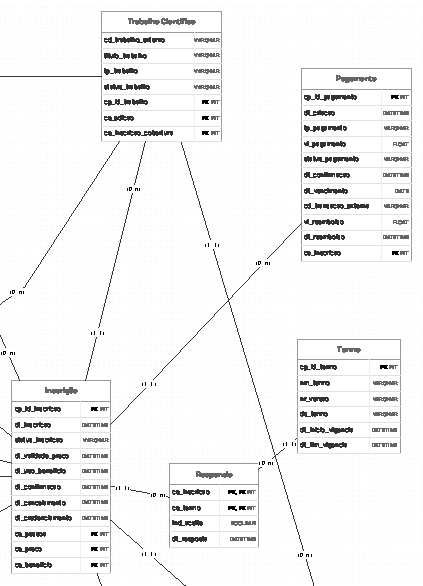
\includegraphics[width=0.8\linewidth]{figura-1-16-logico-parte-f}}
\newcommand{\logG}{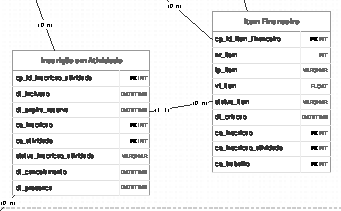
\includegraphics[width=0.66\linewidth]{figura-1-17-logico-parte-g}}

% Cores do brModelo, medidas na exportação do diagrama
\definecolor{brforte}{HTML}{7CC4F8}
\definecolor{brfraca}{HTML}{FFFF88}
\definecolor{brassoc}{HTML}{FCA397}
\definecolor{brauto}{HTML}{79D297}
\definecolor{brrel}{HTML}{F9F9F9}
\definecolor{bratrib}{HTML}{666666}
\tikzset{
  ent/.style={draw=black,line width=0.9pt,minimum width=1.9cm,minimum height=0.62cm,font=\sffamily\scriptsize},
  rel/.style={draw=black,line width=0.9pt,diamond,aspect=2.2,inner sep=1pt,minimum width=1.7cm,font=\sffamily\scriptsize},
  atr/.style={circle,draw=bratrib,line width=0.8pt,minimum size=5pt,inner sep=0pt},
  idt/.style={circle,fill=bratrib,minimum size=7pt,inner sep=0pt},
}
